% ------------------------------------------------------------------------------
% LaTeX Template: Titlepage
% This is a title page template which be used for both articles and reports.
%
% Copyright: http://www.howtotex.com/
% Date: April 2011
% ------------------------------------------------------------------------------

% -------------------------------------------------------------------------------
% Preamble
% -------------------------------------------------------------------------------
\documentclass[paper=a4, fontsize=11pt,twoside]{scrartcl}		% KOMA article

\usepackage[a4paper,pdftex]{geometry}										% A4paper margins
\setlength{\oddsidemargin}{5mm}												% Remove 'twosided' indentation
\setlength{\evensidemargin}{5mm}

\usepackage[english]{babel}
\usepackage[protrusion=true,expansion=true]{microtype}	
\usepackage{amsmath,amsfonts,amsthm,amssymb}
\usepackage{graphicx}
\usepackage[utf8]{inputenc}

% ------------------------------------------------------------------------------
% Definitions (do not change this)
% ------------------------------------------------------------------------------
\newcommand{\HRule}[1]{\rule{\linewidth}{#1}} 	% Horizontal rule

\makeatletter							% Title
\def\printtitle{%						
    {\raggedright \@title\par}}
\makeatother									

\makeatletter							% Author
\def\printauthor{%					
    {\raggedright \large \@author}}				
\makeatother							

% ------------------------------------------------------------------------------
% Metadata (Change this)
% ------------------------------------------------------------------------------
\title{
\includegraphics[height=1.3cm,width=14cm]{CTH_GU_Header} 	% Subtitle of the document
		 	\\[2.0cm]													% 2cm spacing
			\HRule{0.5pt} \\										% Upper rule
			\LARGE \textbf{\uppercase{Population dynamics in an agent based model \\
	with multiple trophic levels}\\
	[0.5cm]
	\large\textit{BSc Thesis in Data- and Information technology}}	% Title
			\HRule{2pt} \\ [0.5cm]								% Lower rule + 0.5cm spacing
			\normalsize \today									% Todays date
		}

\author{
Loanne Berggren \\
Albin Bramstång\\
Henrik Ernstsson\\
Hanna Kowalska Elleberg \\
Erik Ramqvist\\
Sebastian Ånerud\\
[2cm]
Institution for Data- and Information Technology \\
[0.5cm]
\uppercase{Chalmers University of Technology} \\
GOTHENBURG UNIVERSITY \\
Gothenburg, Sweden 2013 \\
BSc project nr 2013:8 \\
}

\begin{document}
%------------------------------------------------------------------------------
% Maketitle
%------------------------------------------------------------------------------
\thispagestyle{empty}				% Remove page numbering on this page

\printtitle									% Print the title data as defined above
  	\vfill
\printauthor								% Print the author data as defined above

\newpage
\tableofcontents
\newpage

\begin{flushleft} 

%------------------------------------------------------------------------------
% Begin document
%------------------------------------------------------------------------------

%------------------------------------------------------------------------------
% INTRODUCTION
%------------------------------------------------------------------------------
\section{Introduction}


%------------------------------------------------------------------------------
% METHODS
%------------------------------------------------------------------------------
\section{Methods}


%------------------------------------------------------------------------------
% THEORY
%------------------------------------------------------------------------------
\section{Theory}

One essential part of this project is to mathematically model how the agents in the system will move and interact with each other. Mathematics is also important in other parts of the application. One example is the graphical representation of agents, when you want to represent an agent as a triangle on the screen, pointing in the direction that the agent is heading.

\subsection{Agent movement and behaviour}

The modelling of agent movement can be done in various ways. In the application the movement of an agent is based on Newton’s laws and equation of motion. The agent is affected by a discrete number of forces and the sum of those forces divided by its mass, determines its acceleration: $$a(t) = F(t)/m$$

For simplicity, the mass of all agents is set to 1. The acceleration is then applied to the agents velocity, which in turn is used to determine the position of the agent in the next timestep t+dt. The forces, accelerations and velocities are all represented by 2-dimensional vectors, since our agents live and interact in a 2-dimensional space. According to Newton's equation of motions the acceleration of an object, is the sum of forces that it is affected by. \newline

There are a discrete number of forces affecting the agents acceleration. The forces an agent can be affected by are the following: \newline

\begin{itemize}
\item Fpred - The force an agent feels from its predator in presence.
\item Fprey - The force an agent feels from its preys in presence.
\item Fenv - The force an agent feels from the environment (e.g. the walls and the obstacles)
\item Fmi - This is the force an agent feels from interacting with nearby neutral agents (agents on same trophic level). The agent is subject to attraction and repulsion from other individuals in a group.
\item Farray - This is the tendency for an agent to equalize its velocity with nearby neutral agents.
\item Fforward - This is the tendency of an agent to keep moving in its current direction.
\item Frandom - The random force that an agent experiences. This can be interpreted as a kind of error in the agents estimation of where to go.
\end{itemize}

The first two forces determines the interaction between predators and preys. The environment force will make sure that no agent is on a position where it cannot be, i.e. outside the 2-dimensional environment, or inside an obstacle. The mutual interaction force, the arrayal force and the forward thrust, are forces that determines how the agent behaves in the presence of other agents of the same population. These are the forces that will determine if the agent wants to group with other agents [A. Okubo, S. A. Levin. (2001)]. The random force is a force that the agent is affected by that can not be properly explained and is therefore said to be random. This could for example be the error the agent does in estimating in what direction it should go. \newline

One can group all the forces into two groups; The the forces explaining the agents own will and the forces an agent have no control over. The predator force, prey force, mutual interaction force, arrayal force, forward thrust and random force are all group as the forces explaining the agents own will. The environment force is a that the agent can not control. An example of this is that an agent chooses to flee from a predator hunting it, but it can not choose to ignore the force of colliding with a wall. \newline

The acceleration of own will ai of an agent is then determined by the following equation:

$$aiown(t) = C1Fpred + C2Fprey + C3Fmi + C4Farray + C5Fforward + C6Frandom$$

where C1,...,C6 are constants weighing the different forces. (Can be interpreted as how much they get influenced by the different forces). \newline

If the norm of the acceleration exceeds the value maxAcceleration for the agent, then the norm is scaled back to maxAcceleration. After the acceleration has been scales, the environment force is applied to the acceleration of own will to form the final acceleration:

$$ai(t) = aiown(t) + C7Fenv$$

where C7 is a constant scaling the force to a propriate value. \newline

The velocity vi an agent has at time t is then given by Newtons equation of motion:

$$vi(t) = vi(t-dt)+ai(t)*dt,$$

If the norm of the velocity exceeds the value maxSpeed for the agent, the norm is scaled to back to maxSpeed. \newline

The position Pi that an agent will have in the next time step t+dt is then the following:

$$Pi(t+dt) = Pi(t)+vi(t)*dt$$

where dt is set to 1 for simplicity. \newline

In the subsections below there will be a more in-depth definition of what the different forces really are and the thoughts behind them.

\subsubsection{Predator force}

The preys wants to find the direction, in what to best escape the predators hunting them. If only one predator is near, the best way to go is straight away from the predator. If there are two or more predators near, the best direction might not be so obvious. \newline

In this project some simplifications have been made, in order to get a closed form solution. Since the maximum distance from all the predators is infinity, this becomes a hard problem. It is easier to solve the problem of finding the position that would minimize the distance to all nearby predators. With the knowledge of that position as a prey, it would make sense to go as far away from it as possible. The problem is now instead of finding the position that would minimize the distance to all nearby predators. The fact that closer predators are more frightening has to be take into account too. \newline

Let di,j denote the distance between the prey i and the predator j and Pi the position of agent i. The vector Fi,j = (Pi - Pj)  is then the vector pointing from the predator to the prey. We then want to find vb that minimizes the norm of the following expression:

$$f(vb) =all nearby j(Fi,j/di,j + vb)$$

Since vb is a 2-dimensional vector with coordinates xb and yb we can take the partial derivatives of f(vb) with respect xb and yb and set them to 0. The xb and yb that satisfies those two equations will be the xb and yb that minimizes ||f(vb)||:

$$df/dx = d((j(xi,j/di,j + xb))^2+(j(yi,j/di,j + yb))^2)/dx = 2n(nxd+Ex)$$ 

where $n > 0$ is the number of nearby predators and Ex = all nearby jxi,j/di,j.

$$df/dy = d((j(xi,j/di,j + xb))^2+(j(yi,j/di,j + yb))^2)/dy = 2n(nyd+Ey)$$ 

where $n > 0$ is the number of nearby predators and Ey = all nearby jyi,j/di,j. \newline

Setting the derivatives to 0 gives:

$$xd = -Ex/n$$

$$yd = -Ey/n$$

$$vb = (xd, yd)$$

The worst position prey i could be in is then Pi + vb. Instead the prey should head in the opposite direction towards Pi - vb. This makes the predator force be the following:

$$Fpred = -vb.$$

This is the weighted average of optimal directions, weighted by the inverse of the distance to the predator. This equation now gives the desired behaviour for preys, when running from predators. Of course this is not the most realistic behaviour of real preys, but it is relatively easy to implement and understand. It also works out well visually. \newline

\subsubsection{Prey force}

To be filled in when a more appropriate force or definition has been applied.

\subsubsection{Environment force}

Since the agents should not move outside the universe, or into any obstacles, there will have to be a way to model how they should interact with the walls and obstacles. One way would be to check at every position update if the new position was valid. But this immediately raises a new question - what to do if the new position is not valid? That solution gave rise to a new and harder problem. Therefore there has to be a better way to handle the interaction with walls and obstacles. \newline

The way this interaction is modelled is again with forces. If an agent is close to the wall, it should feel a force pushing it away from the wall. The closer to the wall an agent is, the greater force it should feel. On the other hand, if the agent is not close enough to the wall, it should not be affected by it. This makes sense since if you are not close enough to a wall or an obstacle, you might not see it. Also if you are running towards a wall, you will come to a point where you would want to stop in order not to run in to the wall. Before that limit, you can still run with maximum speed. \newline

These two features can be modelled in two steps; First the property “the closer the wall, the greater the force” will have to be modelled with a simple and well recognisable function, namely y=1/x. Let y be the magnitude of the force and x be the distance to the wall, and you have a function fulfilling the desired properties. The force should be orthogonal to the wall and pointing into the universe. \newline

The next property to model is that the agents should not feel the force if they are not interacting with the wall. This could be modelled with a simple Heaviside step function (f(x) = 1 if x greater than 0 and = 0 otherwise). A function like that can be seen in Figure X. The direction of the force is the direction of the vector pointing from the closest point on the wall/boundary to the agents position. This is true for the forces an agents feels from both the walls of the universe and the boundary of an obstacle. The equation for the force is then:

$$sum_over_all_obstacles_plus_wall((Pi-Pb)/norm(Pi-Pb)*Heaviside(C-1/x)*1/x).$$


\begin{figure}
\begin{center}
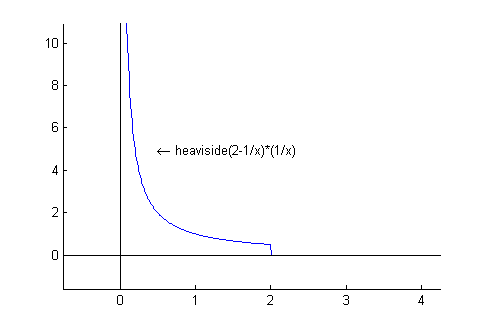
\includegraphics[height=10cm,width=10cm]{heavisideOneDividedByX}
\caption{Shows the Heaviside step function.}
\label{tab:heaviside}
\end{center}
\end{figure}

\subsubsection{Mutual interaction force}

One other desired property of the agent behaviour might be that the neutral agents want to group with each other. Forming a group might improve the agents chances in surviving against predators. The mutual interaction force will make agents far apart steer towards each other to form a group (attraction). At the same time, the agents do not want to collide with each other and will therefore steer away from other agents that are too close (repulsion). The mutual interaction force is defined as:

$$(Fmi)i = j!=iQ(di,j)(Pi - Pj)/di,j$$

where Pi and Pj is the position of the two neutral agents i and j, and Q is a function of the distance between the two agents. Q(di,j) is defined as follows:

$$Q(di,j) = -c0(d0-di,j)$$     

when 0 < di,j < d0 and c0 > 0.

$$Q(di,j) = c > 0$$

when d0  < di,j < dvision

$$Q(di,j) = 0$$
when dvision < di,j. \newline

An agent is then subject to a linearly varying repulsive force from another agent if the distance between the two is less than d0. If the agent is in vision range of another agent, but the distance between them is greater than d0, the agent is subject to a constant attractive force dragging it towards the other agent. If the agents are not in vision range of each other the mutual interaction force is 0 (no interaction).

\subsubsection{Arrayal force} 

The arrayal force describes the tendency of agents in groups to move in the same direction. Two neighbouring agents wants to equalize the velocities in order to steer in the same direction. Without this force, the agents would just form a group where the center of mass is not moving anywhere. The agents are only influenced by other agents that are within a sphere of influence (Vi). This means that an agent does not try to equalize its velocity with other agents that are too far away, even if they are in the same group. The arrayal force that an agent experiences has the following form:

$$(Farray)i = 1/Ni *j in Vih(vi+vj)$$

where Ni are the number of agents within the sphere of influence.

\subsubsection{Forward thrust}

The forward thrust is the tendency of an agent to keep moving in the same direction. The forward thrust is expressed as:

$$(Fforward)i = a*vi/|vi|$$

where a > 0 is a constant called the coefficient of thrust.

\subsection{Finding the closest point on a boundary}

To find the point on the boundary of the universe or an obstacle that is the closest to an agent, is essential when calculating the environment force. In the section for the environment force we assumed that we knew the closest point. In this section different ways of calculating the closest point will be discussed for a subset of geometrical shapes. The obstacles and the universe can be represented as triangular, rectangular and elliptical shapes.

\subsubsection{Triangle}

To be written

\subsubsection{Rectangle/Square}

If the agent is inside the rectangle (rectangular universe), this is the easiest case of them all. All you have to do is to project an agents position onto the sides of the rectangle and then compare which of them are the closest. If the agent is positioned outside the rectangular (rectangular obstacle), this becomes another kind of problem. In Figure X, 8 areas are drawn. Depending on which area the agent is located in, finding closest point differs. If an agent is located in one of the corner areas (1, 3, 5 and 7), the closest point on the rectangle is the closest corner. If the agent is located in any of the other areas, the closest point is given by projecting the agents position onto the closest side of the rectangle.

\subsubsection{Circle}

To find the closest point on the border of the circle, regardless of being inside or outside the it, is simple. The closest point is located on the line that crosses the center of the circle and the agents position. There will be two points on the line that intersects with the boundary of the circle, where the closest one will be chosen.

\subsubsection{Ellipse}

This is by far the most difficult scenario, since there is no closed form solution for the closest point. Instead one has to take a different approach when finding the closest point on an ellipse. Here three different ways will be discussed and evaluated. \newline

The first way of finding the closest point is to do a brute search along the border of the ellipse. Since the equation of the ellipse is known, one can generate N points along its border. This is a really easy way to find a good estimate of the closest point. The downside is that you must have a large N in order to get a precise estimate. Since you will have to do N comparisons to find which is the closest of the N generated points, this algorithm can be computationally heavy, especially when there are a lot of agents doing this calculation every iteration. \newline

A better and faster way is to do a recursive algorithm where you exploit the symmetry of the ellipse. In each iteration of the algorithm you exclude points on the ellipse that you know for sure is not closer than the points already found. In this way you will in each iteration limit the search space and after enough iterations find a good estimate. The algorithm looks as follows:

\begin{enumerate}
\item Initialize starting angle alpha = 0, and step size t = 2*PI/nStep, where nStep is an even integer >= 4.
\item Evaluate nStep points on the ellipse, where the points are (a*cos(alpha+n*t), b*sin(alpha+n*t)) and n = -nStep/2,...,nStep/2.
\item Find the n’ for which the point is closest to the agents position.
\item set newAlpha = alpha + step*n’ and newT = 2*t/nStep
\item got to step 2 with alpha = newAlpha and t = newT, until t is smaller than a stopping value c.
\end{enumerate}

With this algorithm you will do nStep comparisons each iterations and you will stop when t is smaller than e. Since you divide t by nStep/2 in every iteration, you can compute how many iterations the algorithm will run. Let x denote the number of iterations, then the algorithm will stop when $PI*(nStep/2)^{-x}$ is smaller than c. The least number of iterations the algorithm will run is then obtained by solving the following equation for x:

$$PI*(nStep/2)^-x = c.$$

Which gives $x = log(PI/c)/log(nStep/2)$.

Since you will do nStep comparisons each iterations, you will do at a minimum x*nStep comparisons with the algorithm. In Figure X, a plot for x*nStep  as a function of nStep is given. As seen in the figure, for nStep > 2 the function only has one minimum. Taking the derivative of x*nStep and setting it to 0 will give you the minimum of the function:

$$d(x*nStep)/d(nStep) = log(PI/c)*(log(nStep/2) - 1)/(log^2(nStep/2)) = 0$$

Solving the equation for nStep, implies:

$$log(nStep/2) - 1 = 0$$

Which gives nStep = 2*e = 5.44. This means that the optimal choice of nStep is either 4 or 6. To compare this we will take x*nStep when nStep = 6, minus x*nStep with nStep = 4. If the result is negative, then nStep = 6 is the best choice. If the result however is positive, then nStep = 4 is the best choice.

$$6*log(PI/c)/log(6/2) - 4*log(PI/c)/log(4/2) = $$

$$ = log(PI/c)*(6/log(3) - 4/log(2)) = $$

$$ -0.31*log(PI/c)$$.

Since log(PI/c) is positive for c < PI, this gives that nStep = 6 is the best choice for any chosen c < PI. \newline

A good choice of the constant c seems to be 0.01. With c = 0.01 you will get a enough good estimate of the closest point and you will still do it with only log(PI/0.01)/log(6/2) = 5.23, which means that the algorithm will run for 6 iterations with 6 comparisons in each iterations. This gives a total of 36 comparisons in order to find the closest point. The estimate you get when doing a brute search on the boundary only using 36 points is way less accurate than doing the algorithm explained above. \newline

\begin{figure}
\begin{center}
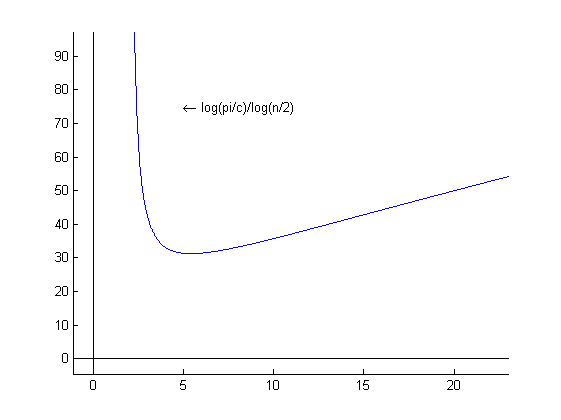
\includegraphics[height=10cm,width=10cm]{recursiveFunctionPlot}
\caption{Showing the number of position comparisons as a function of nStep.}
\label{fig:recursiveFunction}
\end{center}
\end{figure}

The last algorithm comes from a more analytical approach of the problem. The calculations for this algorithm are all taken from (Source). I will here explain the thoughts behind this algorithm. \newline

Let the equation for the ellipse be denoted as:

$$(x/a)^2 + (y/b)^2 - 1 = 0$$

The closest point from an agents position (u, v)  to the ellipse is found where the vector (u-x, v-y) is orthogonal to the gradient of the ellipse. This can easily be understood by drawing a picture. The gradient for an ellipse is:

$$grad((x/a)^2 + (y/b)^2 - 1) = (x/a^2, y/b^2)$$.

The condition for orthogonality then says:

$$(u-x, y-v) = t*(x/a^2, y/b^2)$$

for some value t. In this case, we only need to look at the case where the agent is in the first quadrant (u > 0, v > 0), since the other scenarios can be found out using the symmetry of the ellipse. Also we only need to look at the case where a >= b, since the coordinate system can be transformed to make the ellipse fulfill that. \newline

Solving for x and y gives:

$$x = a^2*u/(t+a^2)$$

$$y = b^2*u/(t+b^2)$$

Putting x and y into the equation of the ellipse grants the following equation:

$$F(t) = (a*u/(t+a^2))^2 + (b*v/(t+b^2))^2 -1 = 0$$

The values for t that satisfies the equation F(t) = 0 gives the candidate solutions for the closest point to (u, v). Since we have put the constraint x > 0 and y > 0, we also need $t > -a^2$ and $t > -b^2$. Since b < a, the constraint for $t > -b^2$ is only needed. \newline

The problem is that F(t) is a rational function which has no closed form solution for t. This gives us two options; Multipy through by the polynominals in the denominator and analyze the roots of the quartic function obtained, or solve the rational equation numerically. In (source) they explain both solutions for the curious person. This report will only cover the latter solution using Newton’s method to approximate the roots. \newline

The first derivative of F is:

$$F’ = …$$

The second derivative of F is:

$$F’ = …$$

If u > 0 and v > 0, F’(t) < 0 and F’’(t) > 0 for all $t belongs to (-b^2, infinity)$. Analysing the limits of the function F(t) when t approaches $-b^2$, gives that F(t) approaches infinity. When t approaches infinity, F(t) approaches -1. This means that F(t) is a strictly decreasing function with only one root in the interval $(-b^2, infinity)$.

To approximate the root t* using Newton’s method is ideal since F(t) is convex in the interval of interest. Given a starting value t0 the iterates of the Newton's method are:

$$ti+1 = ti - F(ti)/F’(ti)$$  for i > 0

The only problem is the choice of t0. An inappropriate choice of t0 can make the algorithm not converge. An initial choice of t0 > t* will lead to a new iterate t1 > t*. If you are unlucky, $t1 < -b^2$ which is outside the domain $(-b^2, infinity)$. Therefore one has to choose t0 for which F(t0) < 0 will guarantee that the algorithm converges to the desired root. A choice of $t0 = b*v - b^2$ fulfills the property of F(t0) < 0 since then $F(t0) = (a*u/(b*v - b^2 + a^2 ))^2 > 0$.

When the root t* is found, the closest point is on the boundary of the ellipse is $(a^2*u/(t*+a^2), b^2*u/(t*+b^2))$.

A quick comparison was made to compare the three different methods. In the comparison the three methods was configured to give approximately the same precision. The time of algorithms was measured when running the each of the algorithms on 10000 randomly distributed points located outside the ellipse and inside a 1000x1000 square. The ellipse itself was located at the coordinates (500, 500) with b = 150 and a = 50. This was then done 100 times to get a good estimate of the mean of the time. Table X reveals the results.

\begin{table}
\begin{tabular}{lll}
Algorithm & Mean of time (ms) & Standard deviaton of time (ms) \\
Brute search (N=700) & 1869.13 & 77.32 \\
Recursive search (nStep = 6, c = 0.01) & 109.30 & 2.63 \\
Newtons method (c = 0.1) & 48.07 & 1.56
\end{tabular}
\caption{Table.}
\label{tab:ellipseComparison}
\end{table}
There is no doubt that Newton’s method is the best, followed by the recursive search with twice the time. Doing a brute search for the takes more than 17 times longer than the recursive search and almost 39 times slower than Newton’s method. The algorithm of choice for this project is clearly Newton’s method.

\subsection{Graphical representation of agents}

To draw objects with OpenGL in java, one must build the objects out of vertex points that forms a polygon. The simplest geometric form is a triangle (not counting lines and points). This makes it the fastest object to draw which is also very desirable. \newline

\subsubsection{Finding the centroid of a triangle}

The problem is then how to draw this triangle given the single position of an agent. The smartest thing would be to draw the triangle with the position of the agent in the center of mass (centroid). In order to find where the center of mass is located in the triangle, we first make the assumption that the triangle must be isosceles. The next step is to mathematically calculate where the center of mass is located. \newline

In Figure X, b is the width of the triangle and h is the height. The centroid of a triangle can be found by drawing lines from the median of each side, to the opposite corner. The triangle's centroid is then located where the lines intersect. Since the triangle is isosceles we already know that the centroid will be located at y = 0. We also only need to draw one line in order to find the centroid. \newline

What we need to do is to find the equation for the line and see in what point it cuts the x-axis. The equation for the line is given by:

$$y = b/2 + k*x$$

$$k = dy/dx = (b/2-(-b/4))/(0-h/2) = -3b/2h$$

Setting y = 0 gives us:

$$b/2 - (3b/2h)*x = 0$$

$$1-(3/h)*x = 0$$

$$3x/h = 1$$

$$x = h/3$$

We have now found that the centroid is located at (h/3, 0). We can also see that the centroid is not affected by the width of the triangle, only by the height. \newline


\subsubsection{The direction of where the triangle points}

We now know where the agents location should be in the triangle, but it is also highly desirable that the triangle points in the direction that the agent is heading. Therefore we also need to take the velocity of the agent into account when drawing the triangle. \newline

In Figure X2, there is five different points drawn. The points Ptop, Pleft and Pright are the points needed in order to draw the triangle with Open GL. I will here explain how to get the these points, given Pcentroid and v. To get from Pcentroid to Ptop we will use the fact that we know that Pcentroid is located at $1/3$ of the height of the triangle. We therefore scale the velocity v to have length $2/3$ of the height and add it to Pcentroid:

$$Ptop = Pcentroid + 2/3 *height*v/norm(v).$$

To get to Pbottom we do a similar thing but instead scale the vector to have length $1/3$ of the height and then subtract it from Pcentroid:

$$Pbottom = Pcentroid - 1/3 *height*v/norm(v).$$

In order to get from Pbottom to Pright and Pleft we need to add a vector that is orthogonal to v and has the length b/2. To form that vector v2, we make use of the fact that the scalar product of two orthogonal vectors are equal to 0:

$$xv*xv2 + yv*yv2 = 0.     (1)$$

and

$$xv22+yv22 = b2/4     (2)$$

solve xv2 from (1) gives:

$$xv2 = -yv*yv2/xv,        xv != 0.$$

Put that into (2) and you get the following:

$$(-yv/xv)2*yv22 + yv22 = b2/4$$

$$yv22(1+(-yv/xv)2) = b2/4$$

$$yv22 = b2/(4*(1+(-yv/xv)2))$$

$$yv2,1  = + b/(2*sqrt(1+(-yv/xv)2)).$$

$$yv2,2  = - b/(2*sqrt(1+(-yv/xv)2)).$$

$$v2 = (xv2, yv2,1) = -v2 = -(xv2, yv2,2)$$

You will get two solutions for yv2 and depending on which of them you choose and the direction of vector v, you will get either Pright and Pleft when you do the addition Pbottom + v2. We do not specifically need to know if Pbottom + v2 is equal to Pright or Pleft. For simplicity in our code, we have made the choice to call Pbottom + v2 for Pright and Pbottom - v2 for Pleft. If it would happen that xv = 0, we can just set yv2 = 0 and xv2 = b/2. \newline

We now have the three points Pbottom to Pright and Pleft, and can draw the triangle in a highly desirable way: The agents position is in the center of mass of the triangle and the top of the triangle pointing is pointing in the same direction as the velocity of the agent. \newline

\begin{figure}
\begin{center}
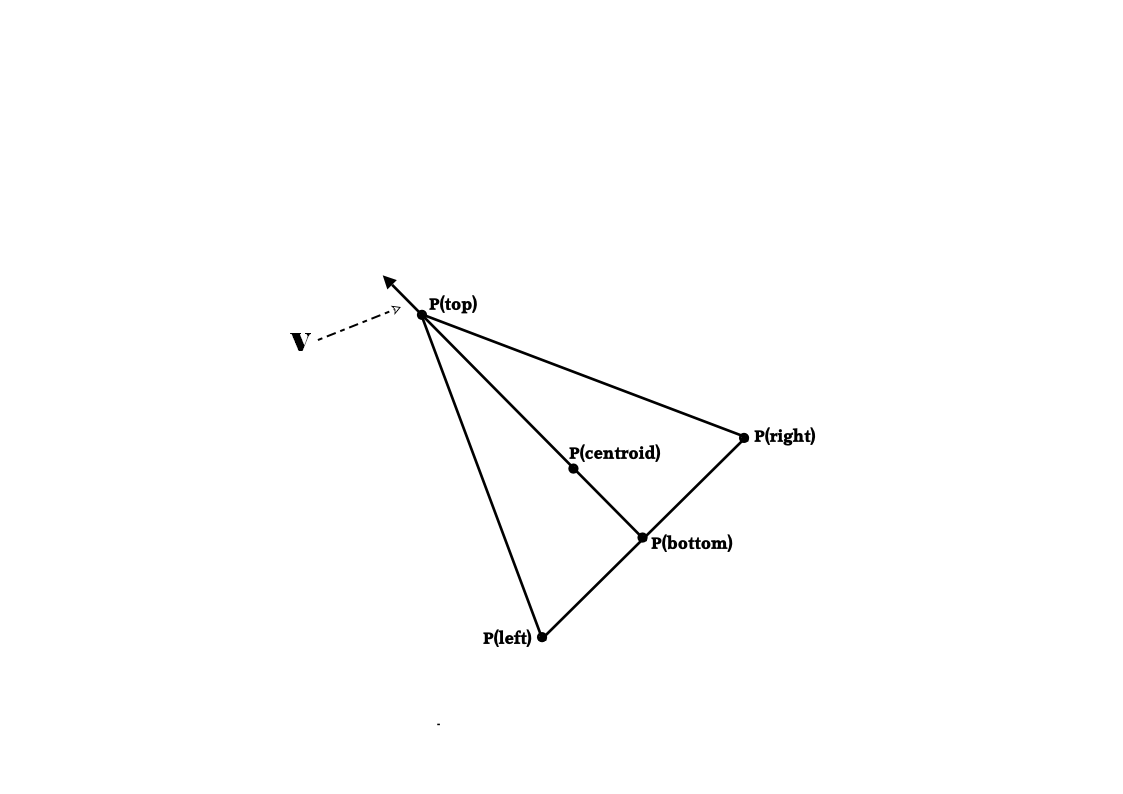
\includegraphics[scale=0.5]{Triangle1}
\caption{Triangle1}
\label{fig:triangle1}
\end{center}
\end{figure}

%------------------------------------------------------------------------------
% RESULTS
%------------------------------------------------------------------------------
\section{Results}


%------------------------------------------------------------------------------
% DISCUSSION
%------------------------------------------------------------------------------
\section{Discussion}


%------------------------------------------------------------------------------
% APPENDIX
%------------------------------------------------------------------------------
\section{Appendix}


%------------------------------------------------------------------------------
% REFERENCES
%------------------------------------------------------------------------------
\section{References}


%------------------------------------------------------------------------------
% End document
%------------------------------------------------------------------------------

\end{flushleft}
\end{document}